\section{Reusable Components}
\label{s:reusable-components}

\begin{figure}
  \begin{lstlisting}
  aprun -n 64 histogram velos.fp 16 velocities &
  aprun -n 256 magnitude lmpselect.fp \
    lmpsel velos.fp velocities &
  aprun -n 256 select dump.custom.fp \
    atoms 1 lmpselect.fp lmpsel vx vy vz &
  aprun -n 1024 lmp_titan < in.cracksm &
  wait
  \end{lstlisting}
  \vspace{-0.15in}
  \caption{SuperGlue example launch script, LAMMPS workflow}
  \label{fig:launch-script}
  \vspace{-0.10in}
\end{figure}

\begin{figure*}
  \vspace{-0.10in}
  \includegraphics[width=\linewidth]{fig/wflow3}
  \vspace{-0.35in}
  \caption{LAMMPS Workflow}
  \label{fig:lammps-workflow}
  \vspace{-0.05in}
\end{figure*}

\begin{figure*}
  %\vspace{-0.10in}
  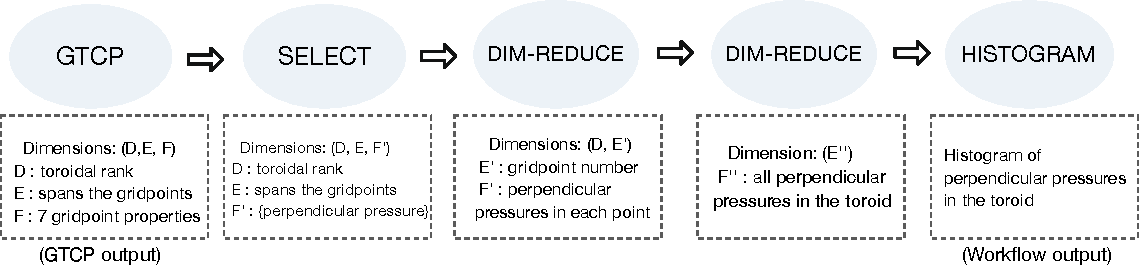
\includegraphics[width=\linewidth]{fig/wflow4}
  \vspace{-0.35in}
  \caption{GTCP Workflow}
  \label{fig:gtcp-workflow}
  \vspace{-0.15in}
\end{figure*}

\begin{figure}
  \center
  %\vspace{-0.10in}
  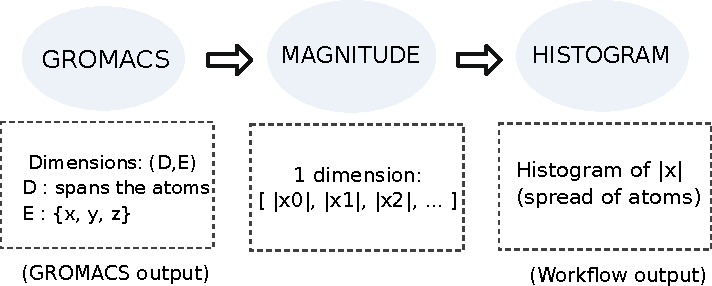
\includegraphics[width=\columnwidth]{fig/wflow_gromacs}
  \vspace{-0.25in}
  \caption{GROMACS Workflow}
  \label{fig:gromacs-workflow}
  \vspace{-0.15in}
\end{figure}



This section provides greater details about the individual SuperGlue components
and how a small number of
parameters allow them to operate on a variety
of different input data formats in
a user-specified way.

\subsection{Select}

Given an input stream that includes an array with
any number of dimensions,
Select extracts certain indices from one of
the dimensions. Thus, it outputs an array
with the same number of dimensions,
but with the dimension of interest having a
smaller size. In order to select the quantities of
interest, the component uses a header which
must be passed by the previous component in the
workflow. The header is a list of strings that
name the quantities in the
dimension of interest. This allows for easy
selection of quantities at runtime when
Select is launched. For example, in the LAMMPS workflow,
the simulation outputs the ID, Type, $v_{x}$, $v_y$, and $v_z$
of each particle, where $v_{x}$, $v_y$, and $v_z$ are the
three-dimensional components of the velocity of a particle.
Select discards the ID and Type, building a new
array consisting only of the velocity components.
The user must pass to
this component the index of the dimension
from which to select, as well as the
indices of the quantities of interest within that dimension.
~\autoref{fig:launch-script} shows an example launch
script for the LAMMPS workflow. Lines 4 and 5
show how Select is launched. \verb|dump.custom.bp|
is the FlexPath stream written by LAMMPS; \verb|atoms|
is the array of atoms written by the simulation; 
1 is the dimension number that spans the 5 atom attributes;
\verb|lmpselect.fp| is the stream that Select will write;
\verb|lmpsel| is the array that Select will write;
\verb|vx| \verb|vy| and \verb|vz| are the
names of the quantities
to be extracted, which will be found in the
header written by LAMMPS.

\subsection{Dim-Reduce}

Dim-Reduce is a glue component that removes one dimension from its
input array, ``absorbing'' it into another dimension without modifying the
total size of the data. The other dimensions are left unchanged. This component
can work with an input array having any number of dimensions. The output is an
array with one dimension removed and with another dimension that has been
re-defined. When using this component, the user must specify which
dimension to eliminate and which to grow.

\subsection{Magnitude}

In our current implementation, Magnitude expects a two-dimensional array as
input, where one dimension spans the data points at each time step (particles
in the case of LAMMPS and grid points in the case of GTC) and the other
dimension spans any number of components of the same vector, for example the
three-dimensional components of velocity in the LAMMPS workflow. Magnitude
calculates the magnitudes of the vectors from the values of their
individual components and outputs
a one-dimensional array of the new values. Which dimension is which in the input
array is specified by the user at runtime. A small number of changes and a few
start-up parameters could generalize this code to perform any number of
common operations that calculate a quantity from many,
applying a known formula over a two-dimensional dataset, thus
allowing this component to be extended into a variety of others.

\subsection{Histogram}

The processes that make up the Histogram component
partition among themselves a one-dimensional
array of data. They communicate to discover the global
minimum and maximum values in the array, create a
number of bins between these two extremes, and
then communicate again to count the number of values in the
globally partitioned array that fall in each bin.
The number of bins to use must be passed to the
component when it is launched.

In our current implementation, one of the processes
of Histogram writes the
output to a file on disk. We chose this approach
because this component is often used as an
endpoint in the workflow and because the output of this
component is generally very small compared to its input
and can be easily written by a single process.
However, letting this component output
its data in the same way as the other components,
that is as an ADIOS stream, and instead writing to
disk when needed using a component specifically
designed for this purpose would
provide greater flexibility.

\subsection{Implementation Details}
The components are implemented as MPI executables
written in C, varying in length from
191 lines of code (Histogram) to
459 (Select).
Their code is publicly available
in~\cite{champsaur:superglue-repo}.


% for future work section
\if 0
\subsection{Dumper}

While this component was not created in time for this paper, the value of
a component specifically designed to be the endpoint of a workflow
is clear. The key goal for this component is to offer a way to write an ADIOS stream into an
output file using some particular format. Whether to write the workflow output as
HDF5, ADIOS-BP, or a simple text file could simply be selected by the user as an option,
requiring no modifications to existing components, and no re-compilation.

Another component that would be of value would be one with a graph plotting capability.
For example, GNU
Plot~\cite{racine:2006:gnuplot} takes a simple text input description and
generates a graph.  Rather than having the graphing component write to
disk, it should also push out an ADIOS stream to some other consumer. An
additional Dumper that writes an image file in a particular format, such as
JPEG, PNG, or SVG, would be a valuable addition.
\fi
